\section{Experiment Definition}\label{sec:definition}
The definition of this experiment is following the GQM (Goal - Questions - Metrics) approach \cite{Basili:1992:SMM:137076}. In this section we define the goal of our experiment, the research questions, and the metrics used to answer those questions.

\subsection{Goal}
\begin{table}[ht]
\centering
\begin{tabular}{||c||} 
\hline
\textbf{Experiment Goal Definition}\\
\hline\hline
Analyze \textbf{native mobile applications \& mobile web applications} \\ 
For the purpose of \textbf{evaluation} \\
With respect to their \textbf{\textcolor{blue}{energy consumption} }\\
From the point of view of \textbf{software users}\\
In the context of \textcolor{blue}{\textbf{the most downloaded applications in Google Play store}}\\ [1ex] 
\hline
\end{tabular}
\caption{Experiment goal of GQM}
\label{tab:goal}
\end{table}
Based on the GQM definition pattern, the experiment goal is defined on Table I:. The goal is to evaluate energy consumption of  native and web applications. The energy consumption of the 5 most popular application pairs will be  monitored, thereafter, if time allows, data from up to 15 pairs of applications will be included. The energy consumption of each trial will be measured 20 times, the mean value of energy consumption for each application will be collected. The browser of choice for web applications is Chrome due to it's popularity\cite{Chromestats}. The popularity of the applications are measured by the number of installations from Google Play. \cite{App_statistics} We are aware that this might give us an biased sample since the most popular applications might have a more or less energy efficient applications relative to general applications. The same reasoning goes for the choice of browser and phone, since Chrome and the phone hardware might be significantly different from other browsers or hardware, this might weaken external validity. \textcolor{blue}{But since we focus on maximizing representativeness and raising the feasibility of the experiment we choose to use the browser and its applications in regard to  popularity.} 
\textcolor{blue}{Finally, the definition of low-end and high-end devices are following the same lines of reasoning as the Mobisoft paper \cite{mobisoft2017}.}

%Further explain why we choose version 6 to be the limit ? 


To summarize, we want to analyze native mobile applications and mobile web applications %..(phone apps and browser apps).. 
for the purpose of evaluation %..(evaluation).. 
with respect to their energy consumption %..(Energy consumption).. 
from the point of view of the software users %..(software developer).. 
in the context of  \textcolor{blue}{ the most downloaded Android applications in Google Play store} %..(Phone usage / thirty phone applications)..?

\subsection{Questions}
Our research embraces 2 research questions:  main research question (RQ1), and 1 additional research question (\textbf{RQ2}). The second question will be explored on the condition that there is enough time.

\textbf{RQ1} - How does energy efficiency differ between native mobile applications and their mobile web counterparts?

To answer to this question, we will have to run the same scenarios on pairs consisting of a native mobile application and its mobile web counterpart. Statistical analysis will be performed to determine whether there is any statistically significant difference.



\textbf{RQ2} - How does the device type affect the difference in energy consumption between native mobile applications and their mobile web counterparts?

To answer this question, we will perform 2 sets of experiments described in \textbf{RQ2}, but one of them has to be on a low-end device, and the other one on a high-end device. Statistical analysis will be performed to determine whether there is any statistically significant difference.


\subsection{Metrics}
We will use the  \textbf{energy \textcolor{blue}{consumption}} to directly answer our research questions. The remaining 3 metrics will supplement our answers with further insight. 
\begin{itemize}
    \item \textbf{Power consumption (W)} - Power consumption of native and web applications while executing the scenario. 	       %measured using Trepn Power Profiler \cite{trepn}.
    \item \textbf{Running time (s)} - total running time of a scenario.
    \item \textbf{Energy consumption (J)} - total energy consumed by running a scenario. Calculated by multiplying the average power consumption and the running time of a scenario.
\end{itemize}
Other metrics would have been possible, for example CPU or memory usage in order to trace the energy consumption of certain applications. However, it would be hard to determine how much the metric would contribute to the energy consumption of the application. Because of that, we decided that these parameters are beyond the scope of this experiment. Some of these metrics however are intrinsically used by the tools that help us find out the metrics we actually do use.
\begin{figure*}[!ht]
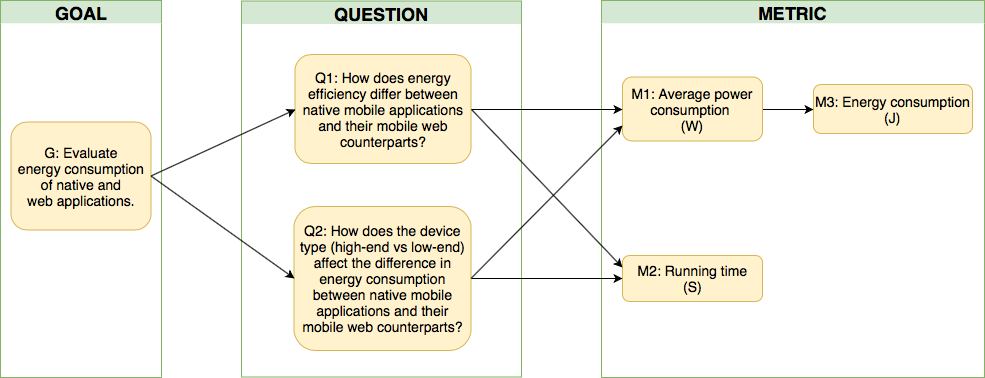
\includegraphics[width=\textwidth]{AppVSweb/figures/GQMtree.png}
\caption{\textcolor{blue}{GQM model hierarchical structure}}
\label{fig:GQMtree}

\end{figure*}
\\To present the experiment idea in a visual way, we picture a GQM tree (\autoref{fig:GQMtree}) based on the elements above.
%\afterpage{\clearpage}

